
\chapter{Drone}

\section{Définition}
La définition suivante est extraite de futura science \cite{futura}.~\\

Un drone est un aéronef sans passager ni pilote qui peut voler de façon autonome ou être contrôlé à distance depuis le sol. Le mot « drone » est employé pour désigner des véhicules aériens, terrestres, de surface ou sous-marins, alors que la classification anglo-saxonne distingue chaque type d’appareil.  ~\\

La taille d’un drone aérien peut aller de quelques centimètres pour les modèles miniatures à plusieurs mètres pour les drones spécialisés (surveillance, renseignement, combat, transport, loisirs). L’autonomie en vol va de quelques minutes à plus de 40 heures pour les drones de longue endurance.  

\section{Type des drones}

On distingue deux types des drones selon leur utilisation et leur taille : militaires et civiles. 

\subsection{Les drones militaires}

Le concept du drone a émergé durant la Premier Guerre mondiale. À l’origine, le drone était un avion-cible à vocation militaire. Son développement a suivi le rythme des grands conflits du XXe siècle : Seconde Guerre mondiale, guerre de Corée, du Vietnam, guerre froide, conflits au Moyen-Orient, guerre d’Irak, d’Afghanistan ou encore en ex-Yougoslavie. Les drones sont plus économiques tout en évitant de mettre en jeu la vie des pilotes et de déployer des troupes terrestres notamment pour les missions de reconnaissance, de surveillance et les attaques ciblées. Leur utilisation au sein des armées et forces de police est devenue prépondérante.  ~\\

% \subsubsection{Types des missions}

 
%En effet, 
Les missions qui leur sont dévolues sont très variées:  ~\\

\begin{itemize}
\item[1.] Écoute des signaux électromagnétiques.
\item[2.]    Observation et surveillance. 
\item[3.]    Détection de missile balistique grâce à une alerte avancée. 
\item[4.]    Relais de communication. 
\item[5.]    Illumination de cibles. 
\item[6.]    Brouillage. 
\item[7.]     Et pour certains, bombardement. 
%\item[8.] Transport de marchandise.
\end{itemize}
 

\subsection{Les drones civils }

Dans le civil, de nombreux domaines (cinéma, télévision, agriculture, environnement, etc.) ont vu les drones susciter des applications inédites grâce à leur capacité à embarquer des appareils photo, des caméras, des caméras infrarouge ou des capteurs environnementaux. Plusieurs sociétés spécialisées dans le transport (DHL, UPS, Allship, La Poste) ainsi que le géant du e-commerce Amazon travaillent sur des concepts de drones-livreurs. Ce type de service a été introduit en 2015 aux Émirats arabes unis pour la livraison de documents officiels.  ~\\

Les drones de loisir ont connu un essor important à partir des années 2010 avec l’arrivée d’appareils miniaturisés, abordables et suffisamment maniables pour être accessibles aux novices. En France, l'utilisation des drones est réglementée par le Code de l’aviation civile, le Code des transports et deux arrêtés émis en 2012. 

%[1]: http://www.futura-sciences.com/magazines/espace/infos/dico/d/aeronautique-drone-6174/ 


    

\section{Fréquence}

Il y a 3 fréquences utilisées pour la communication entre le drone et le télécommande: ~\\
\begin{itemize}
\item 1,3 GHz
\item    2,4 GHz 
\item    5,8 GHz 
\end{itemize}  
~\\


Pour une meilleure qualité d’image, mieux vaut utiliser la bande de 5,8 GHz sachant que le 2,4 GHz permet de plus longues distances mais une qualité d’images plus faible. 

Afin d’éviter les interférences, mieux vaut éviter d’émettre sur la même bande que votre radiocommande. 

Le 2,4 GHz est la même bande que le Wifi, donc à éviter en milieu urbain et en cas d’utilisation évitez d’allumer votre smartphone à côté. 

\section{Types de modulations }

Mais il est impossible d’envoyer un signal numérique tel quel par ondes électromagnétiques. Le signal a besoin d’être modulé, c'est-à-dire transformé d’un signal numérique à un signal analogique. L’opération inverse, la démodulation, se fait par la suite après la réception du signal par la station afin d’obtenir une information exploitable. 

 
\begin{figure}[h]
  \centering
  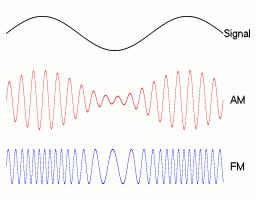
\includegraphics[width=0.7\textwidth]{modulation}
  \caption{types de modulations}
\end{figure}
 


Il existe plusieurs types de modulation dont voici les plus connus: ~\\

 
\textit{AM (Amplitude Modulation) :} Pour faire passer de l’information, on modifie l’amplitude du signal au cours du temps. ~\\

 

\textit{FM (Frequency Modulation) :} Pour faire passer de l’information on modifie la fréquence du signal au cours du temps. ~\\

 

\textit{PM (Phase Modulation) :} C’est la technologie la plus utilisés pour les transmissions radio. Ici on fait passer l’information en modifiant la phase du signal. L’amplitude et la fréquence du signal restent donc fixes. Il existe plusieurs types de modulations par phases : BPSK \footnote{Binary Phase Shift keying}, QPSK\footnote{Quadratic PSK} … BPSK est binaire, on peut donc utiliser deux phases différentes et ainsi faire passer deux types d’informations (0 ou 1). QPSK est quadratique c'est-à-dire que l’on peut utiliser quatre phases différentes donc que l’on peut transmettre quatre types d’informations (00, 01, 10,11). Plus le nombre de phases augmente plus le nombre d’informations pouvant être véhiculé augmente. Mais cela rend le signal plus  exposé aux erreurs car les phases sont de plus en plus proches. ~\\

 

Lorsque l’on modifie la phase d’un signal, on « décale » le signal dans le temps. Graphiquement, cela se traduit par une translation de la courbe du signal sur l’axe des abscisses. La modulation de phase s’exprime en degrés ou en radians. Ainsi 360\up{0} (ou 2n radians) correspond à un décalage d’une période. On dit de deux signaux qu’ils sont en phase lorsqu’ils se superposent. 

 

\begin{figure}[h]
  \centering
  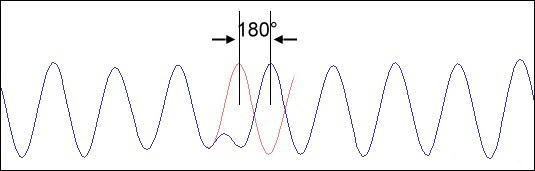
\includegraphics[width=0.7\textwidth]{signal}
  \caption{Exemple d'un signal modulé en phase avec un changement de phase de 180\up{0}}
\end{figure}

 

 

Une fois que ce signal modulé arrive à destination, on opère l’action inverse : la démodulation. Cela permet d’avoir une information numérique exploitable et d’ensuite pouvoir afficher l’image sur un écran afin que le pilote puisse voir ce que drone \og voit \fg{}. 

 

La transmission de données par ondes électromagnétiques ne se fait pas sans erreur, surtout lorsque celles-ci traversent plusieurs milliers de kilomètres dont l'atmosphère terrestre. Ces erreurs surviennent cependant en groupe et de façon très localisé. Mais de simples algorithmes de correction d’erreur comme le FEC\footnote{Forward Error Correction} peuvent assurer de bonnes conditions de transmissions. 

\section{Législations}



La législation en France impose une puissance d’émission maximale de 25 mW dans la fréquence des 5.8 GHz et 100 mW dans la fréquence 2.4 GHz. ~\\

Pour voler en immersion, il faut être 2 avec 2 radiocommandes, un \og esclave\fg{} et un \og maître\fg{} pouvant reprendre le contrôle à tout moment si besoin. ~\\

Les agents de contrôle peuvent, à tout moment, effectuer des contrôles, tant au niveau des utilisateurs amateurs que professionnels, sur le respect des caractéristiques techniques radios des drones. Une utilisation du spectre est trop dangereuse. En cas de non-respect de celles-ci, le matériel peut être saisi et un procès-verbal dressé.~\\ 

Cependant, un arrêté sur les conditions d’utilisation et des personnes capables de  piloter ces drones a été rédigé en France par les services de l’aviation civile le 10 Décembre 2009. Dans l’article 3, les drones doivent être connus des services de l’aviation civile lorsque les drones ne sont pas pour des activités sportives ou récréatives. Ils doivent être connus lorsqu’ils font partie d’une association d’aéromodélisme mais aussi lorsqu’ils évoluent à plus de 150 mètres d’altitudes (ils doivent fournir des justificatifs prouvant le besoin et disposer de précautions particulières, et surtout les vols de nuit ne sont pas autorisés. ~\\

L’utilisation de drones civils est très contraignante. En effet, l’utilisateur doit de demander une autorisation au service de l’aviation civile, pour chaque vol, plusieurs semaines à l’avance ce qui est presque impossible, car les drones dépendent de la météo. De plus, aucune autorisation n’est délivrée à l’heure actuelle pour des survols avec des drones civils dans des zones civiles de zones habitées ou avec un rassemblement de personnes (manifestation). Or, c’est dans ces zones que sont prises la majeure partie des photographies. Il est faux de croire qu’en dessous de 150 mètres d’altitudes il n’y a pas de règlementation et que les avions et hélicoptères avec pilote ne peuvent pas descendre à cette altitude. A cette altitude, il est nécessaire de posséder une autorisation, car sur le territoire français des milliers d’heures de vols se font entre 50 et 150 mètres d’altitudes avec des avions et hélicoptères traditionnels (vols basse altitude d’entrainements militaires, interventions d’hélicoptères de secours).  Les aéronefs traditionnels  ne peuvent pas éviter les drones à cette altitude à cause de leur faible taille, presque invisible en vol. 



%%% Local Variables: 
%%% mode: latex
%%% TeX-master: "rapport_analyse"
%%% End: 
